% \subsection{Motivation}

\begin{frame}{Echo-aware signal processing for audio scene analysis}

    \begin{columns}[T,onlytextwidth]
        \begin{column}{0.65\textwidth}
            \begin{figure}
                \includegraphics<1>[width=\textwidth]{figures/scene1.png}%
                \includegraphics<2>[width=\textwidth]{figures/scene2.png}%
                \includegraphics<3>[width=\textwidth]{figures/scene3.png}%
                \includegraphics<4>[width=\textwidth]{figures/scene4.png}%
                \includegraphics<5->[width=\textwidth]{figures/scene5.png}%
            \end{figure}
        \end{column}
        \begin{column}{0.34\textwidth}
            \textbf{Sound}
            \begin{itemize}
                \item<1-> produced by \alert{sources}
                \item<2-> recorded by (array of) \alert{microphones}
                \item<3-> corrupted by \alert{noise}
                \item<4-> propagates in the \alert{space}
                \item<5-> interacts with the \alert{room}
                          \\$\hookrightarrow$ \alert{reverberation}
            \end{itemize}
            \pause[6]
            $\sum =$ \textbf{Audio Scene}
        \end{column}
    \end{columns}

\end{frame}

\begin{frame}[t]{Echo-aware signal processing for \alert{audio scene analysis}}

    \pause

    \begin{columns}
        \visible<2->{
        \begin{column}[t]{0.3\textwidth}
            \centering
            \alert{Semantic} information

            \vspace*{0.5em}
            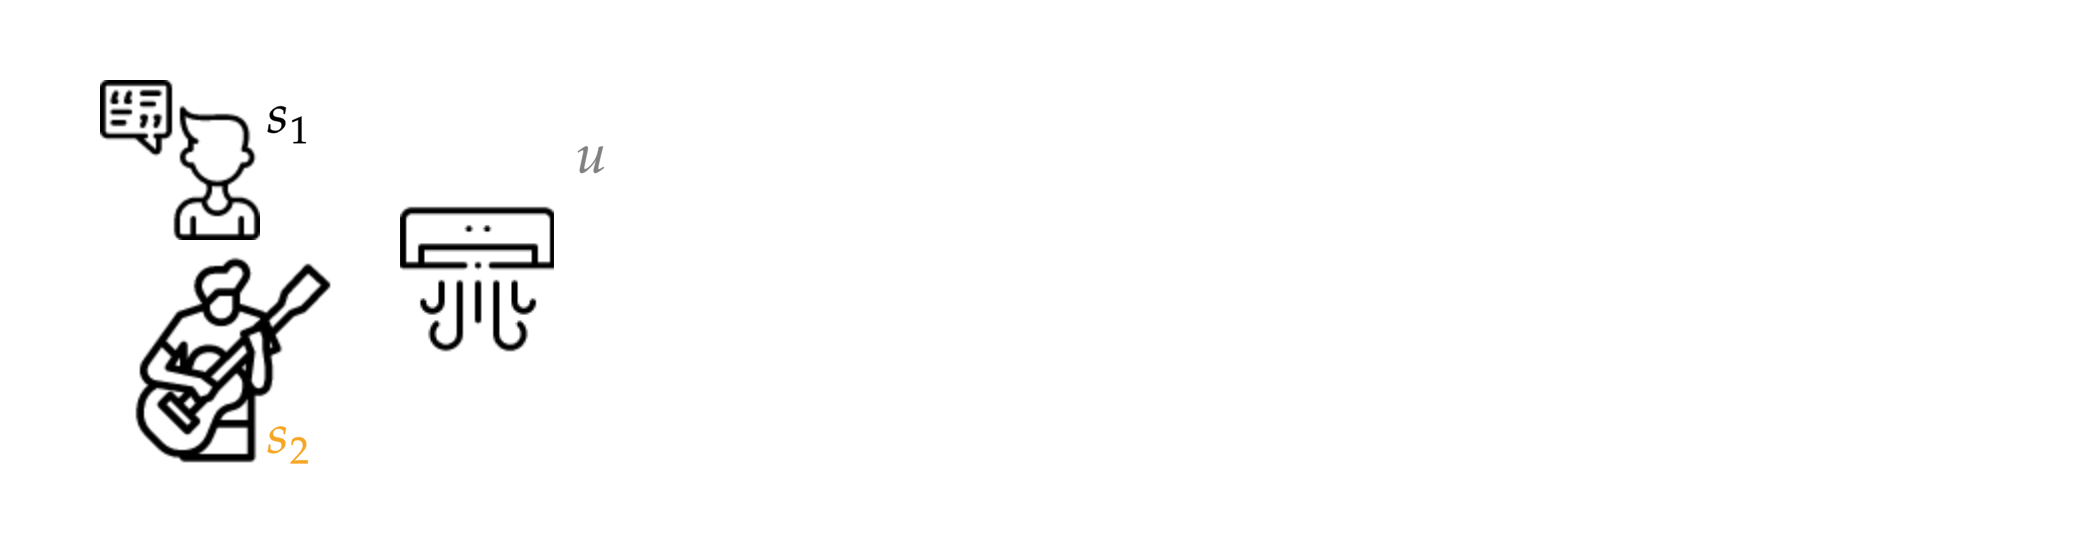
\includegraphics[trim={0 0 170em 0},clip,width=0.7\textwidth]{figures/semantic.png}
        \end{column}}
        \visible<3->{
        \begin{column}[t]{0.3\textwidth}
            \centering
            \alert{Spatial} information

            \vspace*{0.5em}
            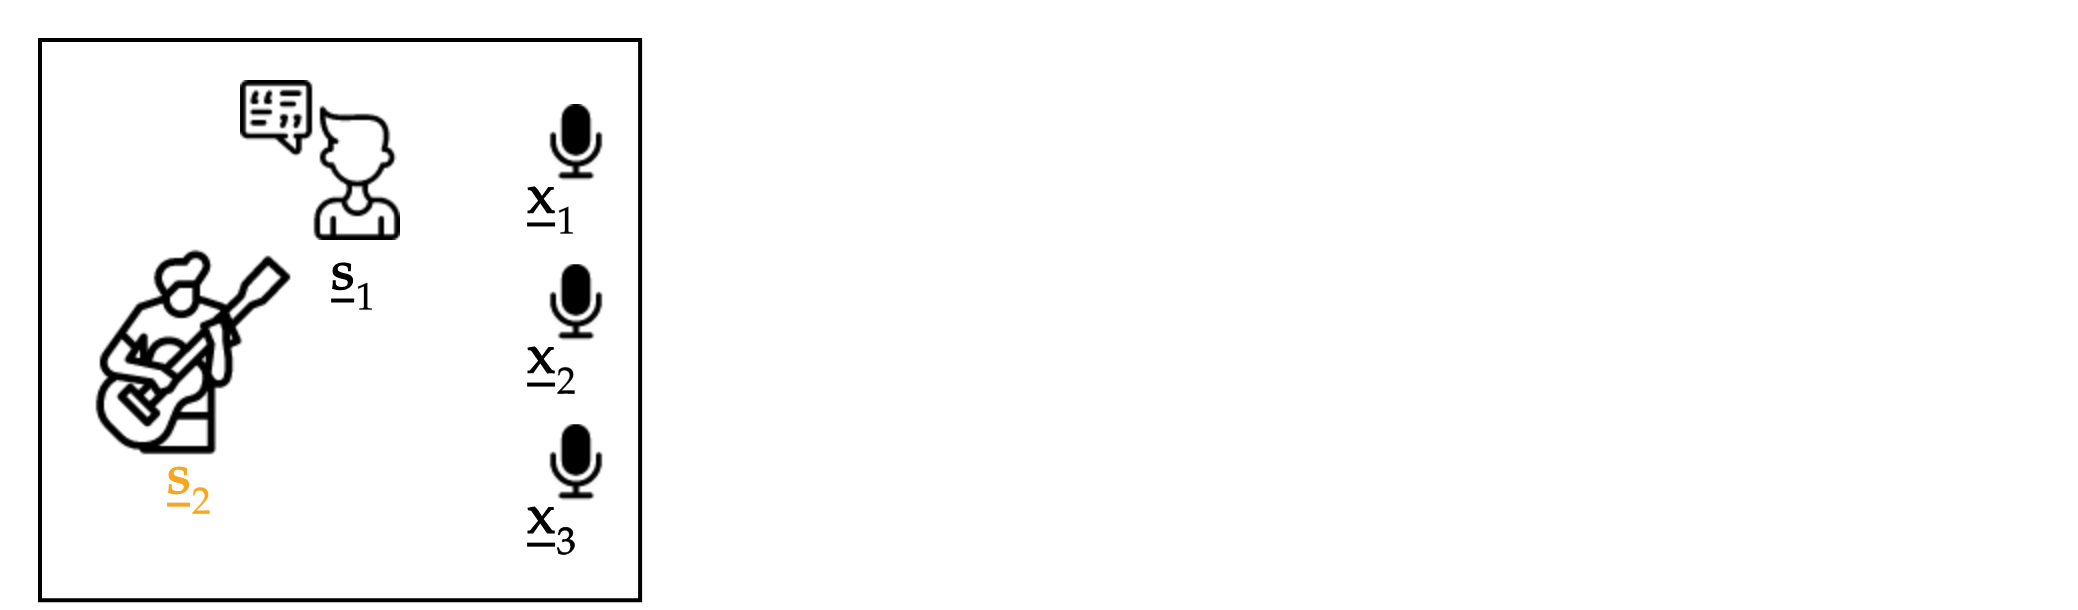
\includegraphics[trim={0 0 170em 0},clip,width=0.7\textwidth]{figures/spatial.png}
        \end{column}}
        \visible<4->{
        \begin{column}[t]{0.3\textwidth}
            \centering
            \alert{Temporal} information

            \vspace*{0.5em}
            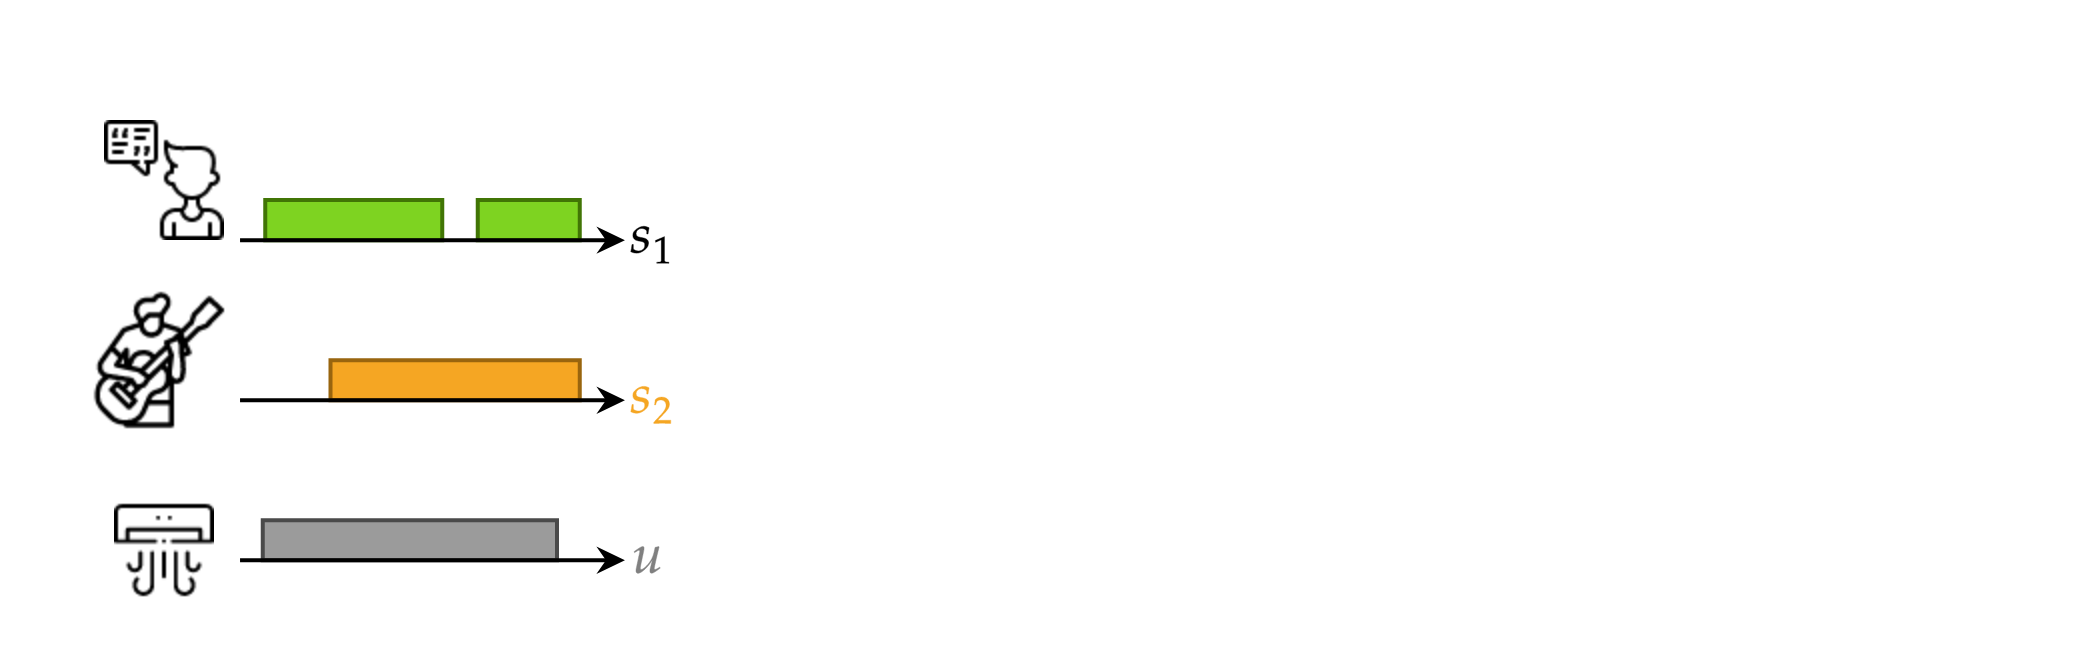
\includegraphics[trim={0 0 170em 0},clip,width=0.7\textwidth]{figures/temporal.png}
        \end{column}}
    \end{columns}

    \begin{columns}
        \visible<2->{
        \begin{column}[t]{0.3\textwidth}
            \centering
            on nature and content
        \end{column}}
        \visible<3->{
        \begin{column}[t]{0.3\textwidth}
            \centering
            on position and geometry
        \end{column}}
        \visible<4->{
        \begin{column}[t]{0.3\textwidth}
            \centering
            on events activity
        \end{column}
        }
    \end{columns}


    \vfill
    \visible<5->{
    \begin{mydefblock}{Audio Scene Analysis}
        Extraction and organization of all the information in the sound
    \end{mydefblock}

    \begin{center}
        \includegraphics<5>[trim={0 35mm 0 35mm},clip,width=0.8\textwidth]{figures/auditory_scene_analysis.png}%
        \includegraphics<6>[trim={0 35mm 0 35mm},clip,width=0.8\textwidth]{figures/scene_analysis.png}
    \end{center}
    }

    \only<6->{
    \begin{textblock*}{40mm}(80mm,90mm)
        \textcolor{myred}{\faRobot~\textbf{Can computers do it?}}
    \end{textblock*}
    }

\end{frame}

\begin{frame}[t]{Echo-aware \alert{signal processing} for audio scene analysis}

    \begin{center}
        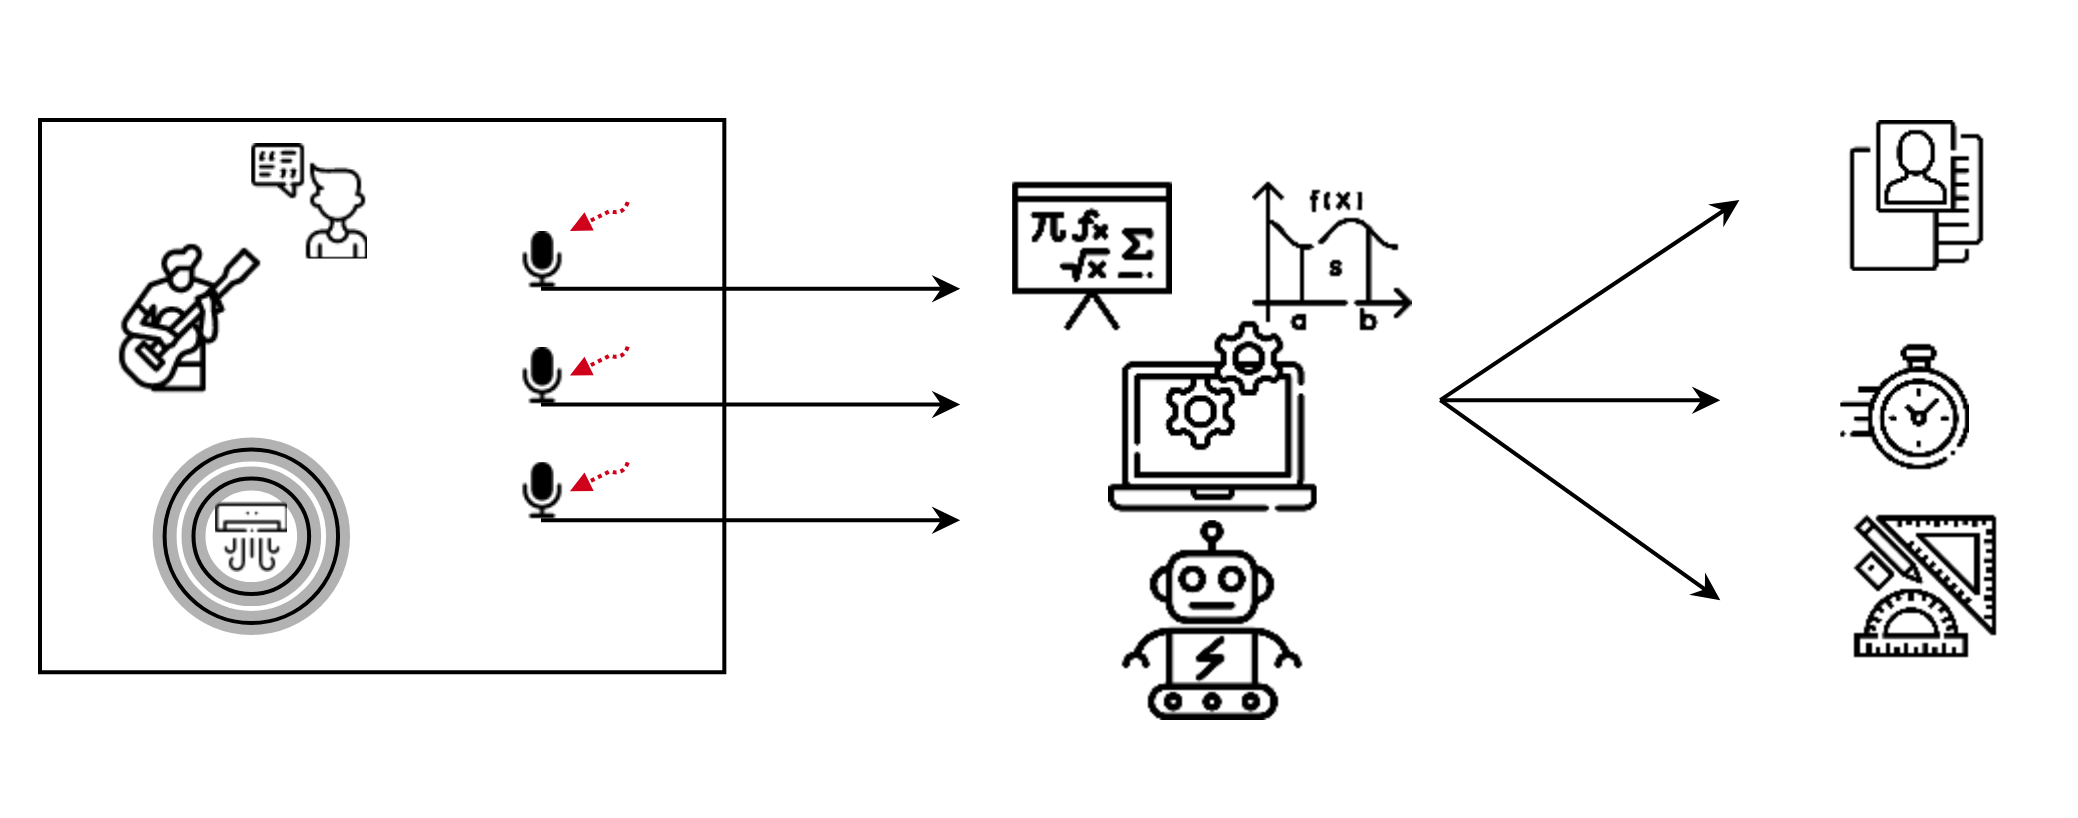
\includegraphics[trim={0 35mm 0 35mm},clip,width=0.8\textwidth]{figures/scene_analysis.png}
    \end{center}

    \pause
    \begin{mydefblock}{Signal Processing}
        Mathematical models, frameworks and tools to tackle and solve such problems
    \end{mydefblock}

    \pause
    \begin{columns}[T,onlytextwidth]
        \begin{column}{0.48\textwidth}
            \small
            \begin{itemize}
                \item Sound Source Separation\tikzmark{top2}
                \item Speech Enhancement\tikzmark{bot2}
                \item Sound Source Localization\hspace{1em}\tikzmark{right1}\tikzmark{top3}
                \item Room Geometry Estimation\tikzmark{bot3}
            \end{itemize}
        \end{column}

        \begin{column}{0.48\textwidth}
            \begin{itemize}\small
                \item Voice Activity Detection\tikzmark{top4}\tikzmark{bot4}
                \item Reverberation level estimation\hspace{1em}\tikzmark{right2}\tikzmark{top5}
                \item Acoustic Channel Estimation\tikzmark{bot5}
                \item ...
            \end{itemize}

    % \begin{columns}[T,onlytextwidth]
    %     \begin{column}{0.48\textwidth}
    %         \footnotesize
    %         \begin{itemize}
    %             \item Speaker Identification\tikzmark{top1}\tikzmark{bot1}
    %             \item Sound Source Separation \tikzmark{top2}
    %             \item Speech Enhancement
    %             \item Automatic Speech Recognition\hspace{0.5em}\tikzmark{right1}\tikzmark{bot2}
    %             \item Sound Source Localization \tikzmark{top3}
    %             \item Room Geometry Estimation \tikzmark{bot3}
    %         \end{itemize}
    %     \end{column}

    %     \begin{column}{0.48\textwidth}
    %         \begin{itemize}\footnotesize
    %             \item Voice Activity Detection\tikzmark{top4}
    %             \item Diarization                \tikzmark{bot4}
    %             \item RT$_{60}$ estimation       \tikzmark{top5}
    %             \item Acoustic Channel Estimation\hspace{0.5em}\tikzmark{right2}
    %             \item Wall Absorption Estimation\tikzmark{bot5}
    %             \item ...
    %         \end{itemize}

        \end{column}
    \end{columns}

    % \begin{tikzpicture}[overlay, remember picture]
    %     \node[anchor=base] (a) at (pic cs:top1) {\vphantom{h}}; % push the mark to the top of the line (ie including ascenders)
    %     \node[anchor=base] (b) at (pic cs:bot1) {\vphantom{g}}; % push the mark to the bottom of the line (ie including descenders)
    %     \draw [decoration={brace,amplitude=0.5em},decorate,thick,gray]
    %      (a.north -| {pic cs:right1}) -- node[right,inner sep=1em] {\small Who?} (b.south -| {pic cs:right1});
    % \end{tikzpicture}
    \begin{tikzpicture}[overlay, remember picture]
        \node[anchor=base] (a) at (pic cs:top2) {\vphantom{h}}; % push the mark to the top of the line (ie including ascenders)
        \node[anchor=base] (b) at (pic cs:bot2) {\vphantom{g}}; % push the mark to the bottom of the line (ie including descenders)
        \draw [decoration={brace,amplitude=0.5em},decorate,thick,gray]
         (a.north -| {pic cs:right1}) -- node[right,inner sep=1em] {\small What?} (b.south -| {pic cs:right1});
    \end{tikzpicture}
    \begin{tikzpicture}[overlay, remember picture]
        \node[anchor=base] (a) at (pic cs:top3) {\vphantom{h}}; % push the mark to the top of the line (ie including ascenders)
        \node[anchor=base] (b) at (pic cs:bot3) {\vphantom{g}}; % push the mark to the bottom of the line (ie including descenders)
        \draw [decoration={brace,amplitude=0.5em},decorate,thick,gray]
         (a.north -| {pic cs:right1}) -- node[right,inner sep=1em] {\small Where?} (b.south -| {pic cs:right1});
    \end{tikzpicture}
    \begin{tikzpicture}[overlay, remember picture]
        \node[anchor=base] (a) at (pic cs:top4) {\vphantom{h}}; % push the mark to the top of the line (ie including ascenders)
        \node[anchor=base] (b) at (pic cs:bot4) {\vphantom{g}}; % push the mark to the bottom of the line (ie including descenders)
        \draw [decoration={brace,amplitude=0.5em},decorate,thick,gray]
         (a.north -| {pic cs:right2}) -- node[right,inner sep=1em] {\small When?} (b.south -| {pic cs:right2});
    \end{tikzpicture}
    \begin{tikzpicture}[overlay, remember picture]
        \node[anchor=base] (a) at (pic cs:top5) {\vphantom{h}}; % push the mark to the top of the line (ie including ascenders)
        \node[anchor=base] (b) at (pic cs:bot5) {\vphantom{g}}; % push the mark to the bottom of the line (ie including descenders)
        \draw [decoration={brace,amplitude=0.5em},decorate,thick,gray]
         (a.north -| {pic cs:right2}) -- node[right,inner sep=1em] {\small How?} (b.south -| {pic cs:right2});
    \end{tikzpicture}

    \pause
    \begin{center}
        \tikzmarknode{how}{HOW}  $\xrightarrow{\textit{helps}}$ WHERE
            $\xrightarrow{\textit{helps}}$ WHAT
            $\xrightarrow{\textit{helps}}$ HOW
            $\xrightarrow{\textit{helps}}$ \tikzmarknode{again}{...}
    \end{center}

    % \pause
    % \begin{tikzpicture}[overlay,remember picture,
    %     nodes={inner sep=1pt, align=center, font=\footnotesize},
    %     gray!70,>=stealth] %
    % \draw[->] (again.south) to[out=-90, in=-90] (how.south);
    % \end{tikzpicture}

\end{frame}


\begin{frame}[t]{\alert{Echo-aware} signal processing for audio scene analysis}

    \begin{columns}[onlytextwidth]
        \column{0.55\textwidth}
        \begin{block}{Sound interacts with indoor environment:}
            \small
            \begin{itemize}
                \item[] it is reflected\tikzmark{topA}
                \\\hspace{1em} specularly and diffusely\hspace{1em}\tikzmark{rightA}
                \item[$+$] it is absorbed,
                \item[$+$] it is transmitted,
                \item[$+$] it is diffracted, etc.\tikzmark{botA}
            \end{itemize}
        \end{block}

        \column{0.55\textwidth}
        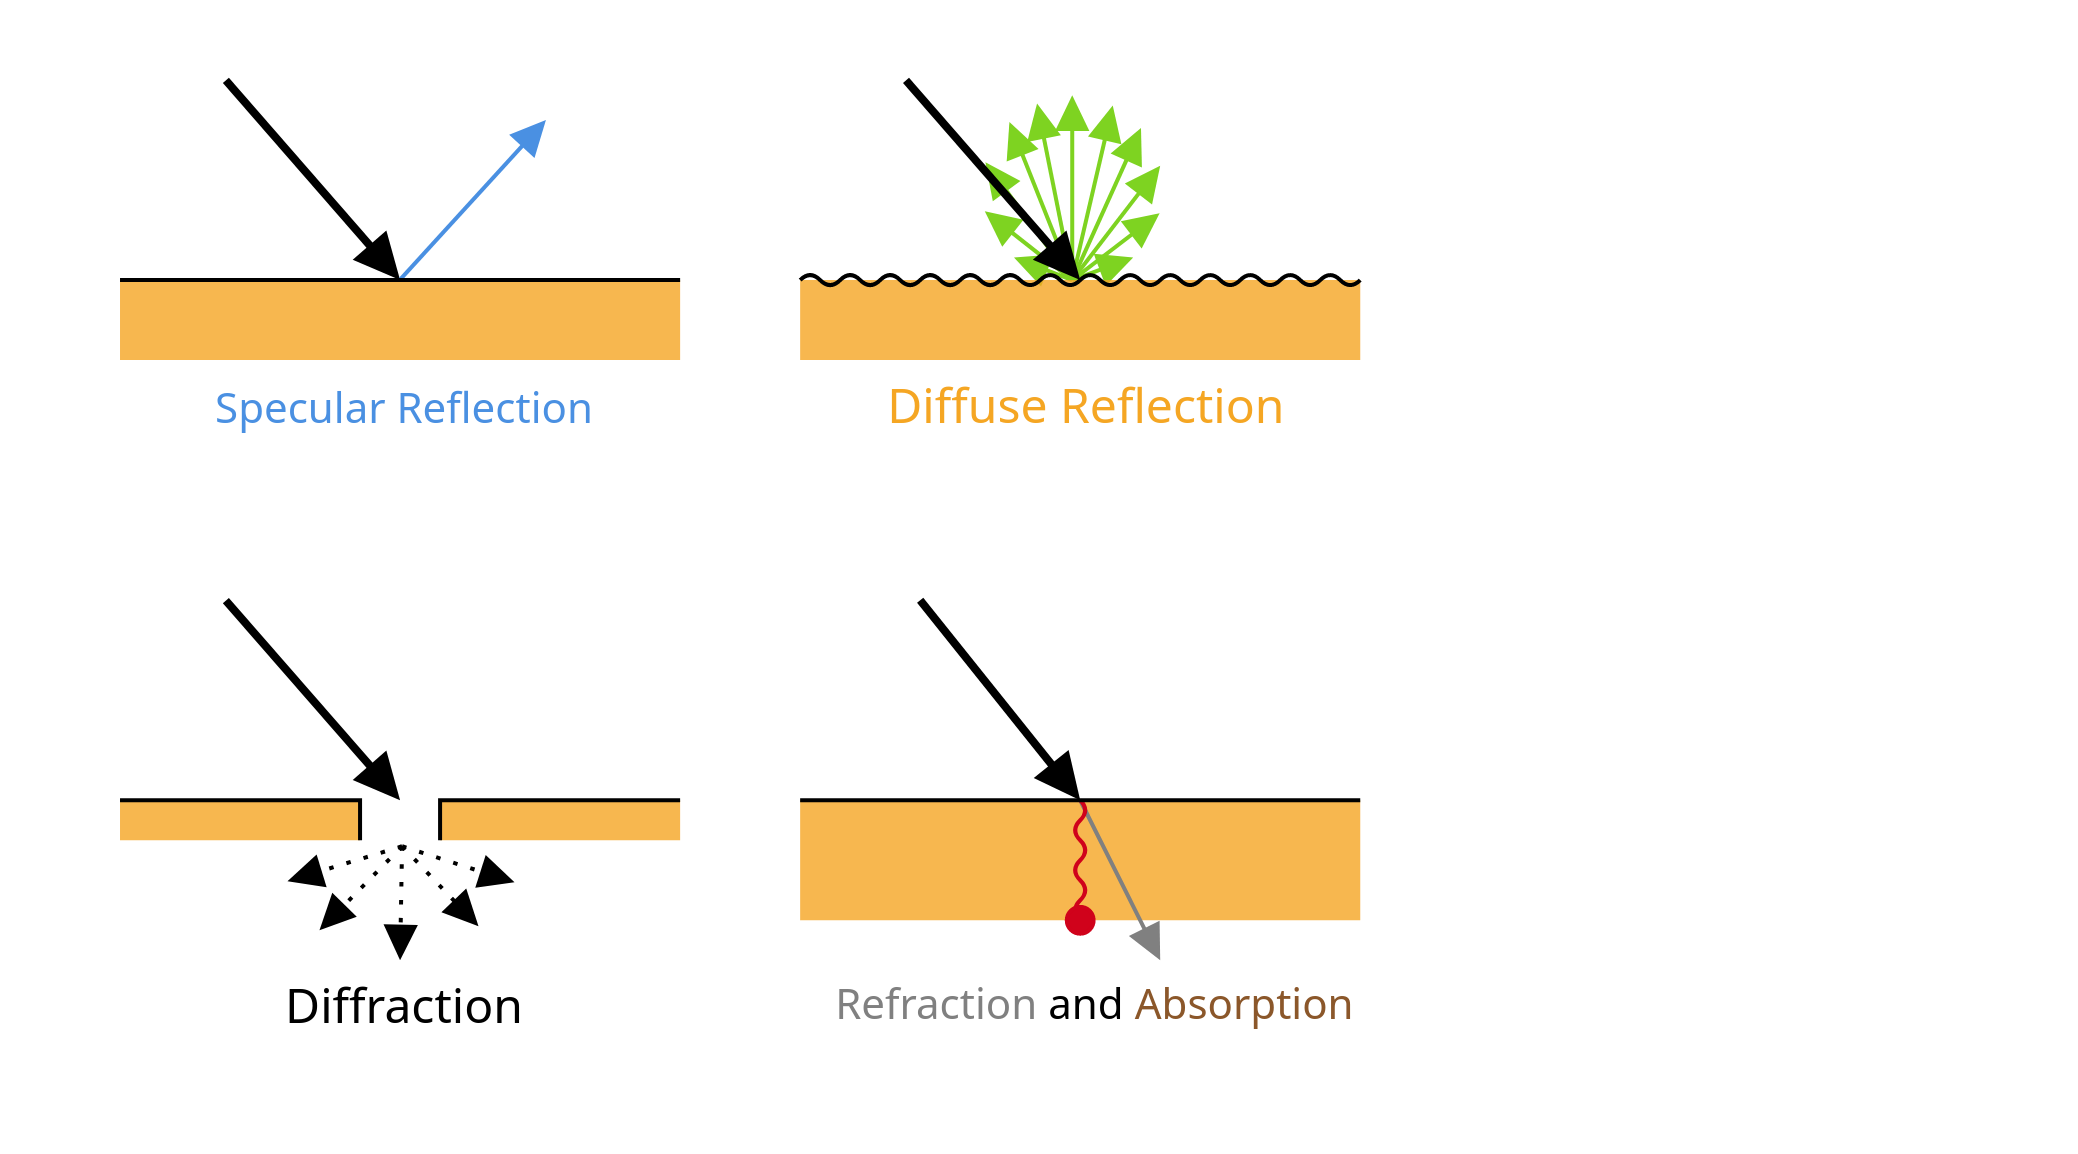
\includegraphics[trim={0 0 50 0},clip,width=\textwidth]{figures/sound_refletion.png}
    \end{columns}

    \pause
    \begin{tikzpicture}[overlay, remember picture]
        \node[anchor=base] (a) at (pic cs:topA) {\vphantom{h}}; % push the mark to the top of the line (ie including ascenders)
        \node[anchor=base] (b) at (pic cs:botA) {\vphantom{g}}; % push the mark to the bottom of the line (ie including descenders)
        \draw [decoration={brace,amplitude=0.5em},decorate,thick,gray]
            (a.north -| {pic cs:rightA}) -- node[right,inner sep=1em]
                {{\small $=$ reverberation}}
            (b.south -| {pic cs:rightA});
    \end{tikzpicture}

    \pause
    \begin{mydefblock}{Acoustic Echoes: early specular reflection}

        \vspace{-2mm}
        \begin{columns}[onlytextwidth]
            \begin{column}{0.58\textwidth}
                \begin{itemize}
                    \item Reflections ``standing out'' w.r.t. reverberation
                    \item Copy of a sound but later
                    \begin{itemize}
                        \item same content
                        \item delay $\Leftrightarrow$ travelled distance
                    \end{itemize}
                \end{itemize}
            \end{column}
            \begin{column}{0.40\textwidth}
                \centering
                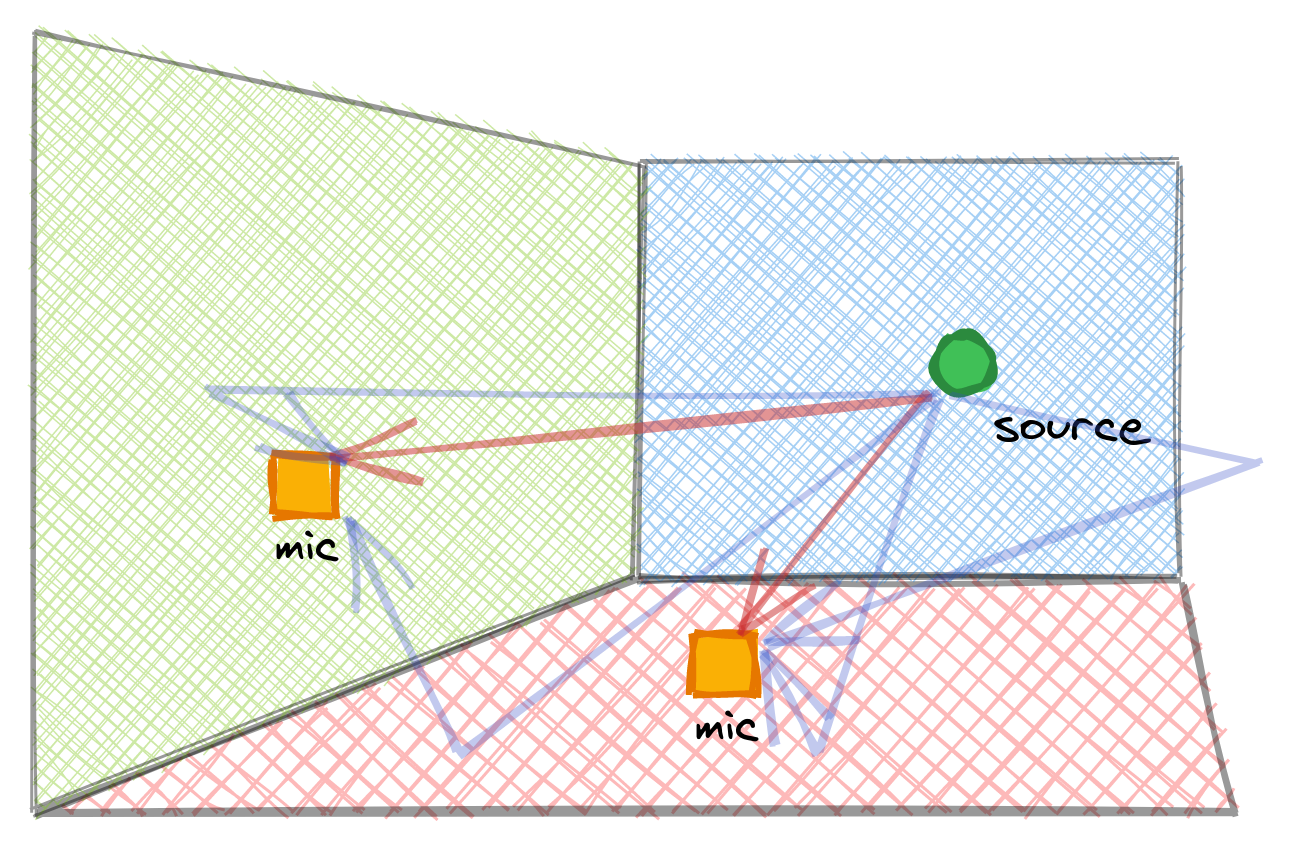
\includegraphics[width=\textwidth]{figures/echoes}
            \end{column}

        \end{columns}
    \end{mydefblock}

    \pause
    \begin{center}
        \faExclamation~\textbf{idea:} leverage this
    \end{center}
\end{frame}

\begin{frame}[t]{\alert{Echo-aware} signal processing for audio scene analysis}

    \textbf{Everyday examples:} bats, dolphins and sonars

    \begin{center}
        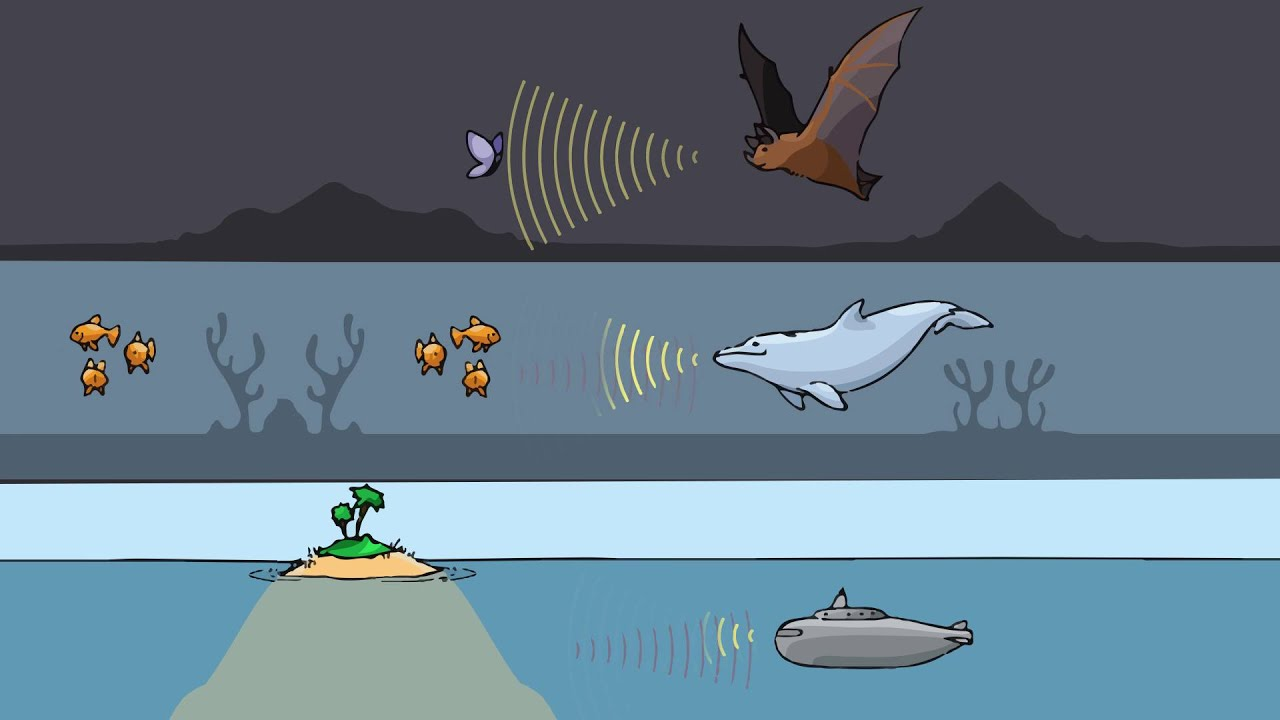
\includegraphics[width=\textwidth]{figures/echo_nature.jpg}
        \addendum{\small\faCopyright[regular]~Skin \& Bones}
    \end{center}

\end{frame}

\begin{frame}{\alert{Echo-aware} signal processing for audio scene analysis}


    \begin{block}{}
        In audio signal processing, sound propagation is typically
        \begin{itemize}
            \item \alert{ignored} $\implies$ simple processing but reverberation is noise
            \item \alert{fully modeled} and estimated $\implies$ very challenging
        \end{itemize}
    \end{block}

    \pause
    \begin{mydefblock}{Echo-aware methods}
        \begin{itemize}
            \item explicitly account for some acoustic reflections to boost the performance
            \item attractive alternative between ignoring reverberation and modelling it entirely
        \end{itemize}
        \begin{center}
            \textit{Turning Enemies into Friends:
            \\Using reflections to improve sound source localization.}
        \end{center}
        \hfill \cite{ribeiro2010turning}
    \end{mydefblock}



\end{frame}

\subsection*{Outline and Contribution}

\begin{frame}{Outline and contributions}

    \begin{block}{Thesis title:}

        \vspace*{2mm}
        \begin{columns}[onlytextwidth]
            \begin{column}[T]{0.3\linewidth}
                \centering
                \visible<2->{
                    \alert{Echo-aware}
                \\\downarrow
                \\better processing

                }
            \end{column}\hfill
            \begin{column}[T]{0.3\linewidth}
                \centering
                \visible<3->{
                \alert{Signal Processing}
                \\\downarrow
                \\models and frameworks
                }
            \end{column}\hfill
            \begin{column}[T]{0.3\linewidth}
                \centering
                \visible<4->{
                \alert{for Audio Scene Analysis}
                \\\downarrow
                \\context and problems
                }
            \end{column}\hfill
        \end{columns}
    \end{block}

    \visible<5->{
    \begin{block}{Thesis contribution:}

        \vspace*{2mm}
        \begin{columns}[T,onlytextwidth]

            \begin{column}{0.48\textwidth}
            \centering
            \alert{1. How to estimate them?}
            \visible<6->{
            \begin{itemize}
                \item Learning-based method
                \item Analytical method
            \end{itemize}}
        \end{column}
        \begin{column}{0.48\textwidth}
            \centering
            \alert{2. How to use them?}
            \visible<7->{
            \begin{itemize}
                \item Source Localization
                \item Speech Enhancement
                \item \textcolor{gray!80}{Source Separation}\addendum{\small in the \faBook}
                \item \textcolor{gray!80}{Room Geometry Estimation}\addendum{\small in the \faBook}
            \end{itemize}}
        \end{column}
    \end{columns}
    \end{block}

    \vspace{2mm}
    \begin{columns}
        \column{0.5\textwidth}
        \centering
        \alert{3. Where to find them?}
        \visible<8->{
            \begin{itemize}
                \item Echo-aware database
            \end{itemize}}
    \end{columns}
    }
\end{frame}